\documentclass[a4paper,10pt]{report}
\usepackage[colorlinks=true,urlcolor=blue,citecolor=black,linkcolor=black,bookmarks=true]{hyperref}
\usepackage{caption}
\usepackage[utf8x]{inputenc}
\usepackage{graphicx}
\usepackage[hmargin=3cm,vmargin=3cm]{geometry}
\usepackage{listings}
\usepackage{enumerate}
\usepackage{algorithmic}
\usepackage{algorithm} 
\usepackage{todo}
\usepackage{float}
%opening
\title{}
\author{simon}
\begin{document}

\chapter{Medea Specialize}

This project have been made to test if swarm of robotic agents are able to split in two different subpopulations which use different ressources.


\section{Energy and Foraging}


\subsection{Energy Point}
In order to survive, agents have to passe on "ressource" patches. Those ressources are implemented as MedeaSpEnergyPoints, stored as InanimatedObject. They have a $type$ which can be 0 or 1 ; and a quantity of energy available ($Q_E$), which said how many "items" can be taken, knowing that each agent can take only one item per iteration (if it remains any items on the ressource). The quantity available is set by the gNbAllowRobots variable in the propertes file. After each iteration $Q_E$ is set back to $gNbAllowRobots$.

Summary :
\begin{enumerate}
 \item $type \in \{0,1\}$,
 \item $gNbAllowRobots$ to set the number of robots that can take a ressource. 
 % item on the energy point of type 1 at each iteration. Energy Points of type 0 allow 100 - gNbAllowRobots. 
 \begin{algorithmic}
 \IF {$type=1$} 
 \STATE $ Q_E \leftarrow gNbAllowRobots $ 
 \ELSE 
 \STATE $Q_E \leftarrow 100 - gNbAllowRobots$
 \ENDIF
 \end{algorithmic}
 \item 
 
\end{enumerate}


\subsection{Agent's foraging abilities}
Agent owe a gene ($g_{skill}$) which is a double $\in\left[-1,1\right]$.




\section{Ressources and robots positions}
\subsection{With movements}
Experiments with movement allow Robots and ressources to move. To execute those experiments you should setup $gExperimentNoMovement = true$.
The position of the two suns will be updated each : $gSunLifetime$. 

The choice of the position of the sun after each $gSunLifetime$ can be setted in two different ways:


\subsubsection{Randomly }
To activate this setup you should put :
$$ gRandSun = true$$

Note : the file medea-sp.properties is an example of a config file to test that kind of experiments. The specialisation in this case doesn't work but robots are able to follow the sun.

In this setup the two suns move randomly in all the area. 

\subsubsection{fixed path}
To activate this setup you should put :
$$ gRandSun = false$$

In this setup the two suns follow an eight like path. Each sun start at the center of the eight, afterwhat they move in opposite directions. 

The path is divided in 14 points drawing a "8" (cf. figure \ref{fig:8like}). The coordinates of those 14 points are hardcoded in MedeaSpWorldObserver.cpp. Two other arrays also hardcoded in MedeaSpWorldObserver.cpp give in which order the sun will jump point two point, thus describing the loop each sun will follow. The current loop is made by 16 moves, but other loop are available in MedeaSpWorldObserver.cpp file

\begin{figure}[H]
\caption{Allowed positions of energy points during simulation (numbers are just id, not an order)}
\label{fig:8like}
\centering
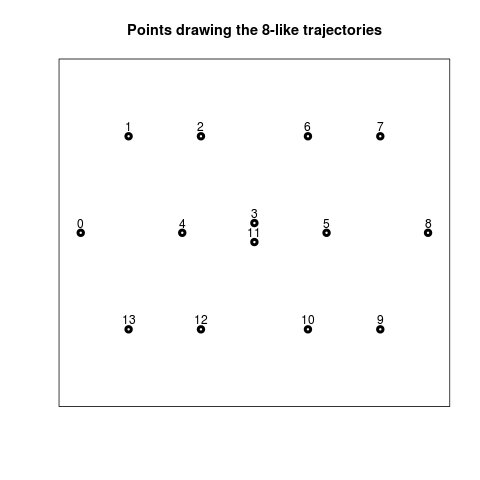
\includegraphics[width=.5\textwidth]{../images/traj8like}
 \end{figure}

% Remarque : the current loop are build in a way that the two suns meet themselves at the center of the area. It looks like when these meeting occurs  


\subsection{With fixed communication network} 
In those cases robots and suns will not move ; so to activate those kind of setup $gExperimentNoMovement$ should be $true$.

\subsubsection{5 topologies:}

Five different topologies based on :
\begin{description}
\item[ Two resources dispositions ]:
\begin{enumerate}[R1.]
\item La moitié des robots + 1 peut atteindre les deux ressources, l'autre moitié +1 peut atteindre l'autre ressource,  \label{it:1acc}
\item Les deux ressources accessibles par tous les robots.\label{it:2acc}
\end{enumerate}

\item[	Two robots dispositions]:
\begin{enumerate}[B1.]
\item Les robots sont en ligne et ne communiquent que deux à deux. \label{it:ligne}
\item La population de robots est constituée de deux sous groupes qui ne peuvent communiquer entre eux que par le biais de deux robots. Au sein des sous groupes tous les robots peuvent communiquer.
.\label{it:2gp}
\end{enumerate}
\end{description}

Which made five environnement:
\begin{table}[h]
\begin{tabular}{l|c|c|}
$gExperimentNumber$&robot disposition& ressources disposition: \\
\hline
0 &tous les robots communiquent & \ref{it:2acc}\\\hline
1 &B\ref{it:ligne} & R\ref{it:2acc}\\\hline
2 &B\ref{it:ligne} & R\ref{it:1acc} \\\hline
3&B\ref{it:2gp} & R\ref{it:2acc}\\\hline
4&B\ref{it:2gp} & R\ref{it:1acc} 
\end{tabular}
\end{table}

To active one of those 5 environnements you just have to set $gExperimentNumber$ with the right number (and be sure that $gExperimentNoMovement$ is $true$). 
\subsubsection{Static network with given sparsity}
\label{sec:staticnet}
Il est possible de choisir arbitrairement quels robots pourront communiquer avec quels autres, sans passer par la radio des robots. Pour utiliser cette configuration il suffit de changer d'initialiser dans le fichier de properties : $gRadioNetwork = false$. Suite à quoi la matrice de communication sera initialisée arbitrairement de fa\c con totalement independant de la position des robots.

La classe $MedeaSpNetworkGenerator$ permets de générer des reseaux aléatoire avec une sparsité donnée et d'initialiser la matrice de communication en fonction de se réseau. Le choix de la sparsité se fait en ajuste la variable $gSparsity$ dans le properties file. En sachant que la variable dans le propertie file est donnée directement en pourcent (ie$gSparsity = 20$ signifie que la classe MedeaSpNetworkGenerator va généré un réseau avec une sparsité de 20\%, ou de 0.20)

Il est aussi possible d'écrire dans un fichier le graphe au format .dot, format lisible par les outils GraphViz qui en permettent la visualisation (cf section\ref{sec:visualisation}).

\section{Fichier de sorties et Logs}
\begin{itemize}

\item datalog\_\$\{dateexpe\}.txt\footnote{\$\{dateexpe\} est la date à la micro seconde à laquelle a été lancée l'expérience} Les fichiers de log principaux, qui contiennent : 
\begin{itemize}

\item les actifs à chaque $n$ iteration (avec $n == gLifeTime$, attention car cela ne veut pas dire qu'à la fin de chaque génération le nombre d'actifs est loggé car les générations ne sont pas synchronisées!) et leur repartition entre ceux capable de prendre la ressource 0, la ressource 1 ou les deux. Codé dans MedeaSpWorldObserver.
 \item lors de la selection d'un nouveau génome : l'identifiant du père à qui appartient le génome sélectionné. Codé dans MedeaSpAgentObserver.cpp
 \item lorsqu'un agent est activé : la valeur du gène capable de se spécialiser et le lieu où l'activation se fait. Codé dans MedeaSpAgentObserver.cpp
\end{itemize}

\item properties\_\$\{dateexpe\}.txt : le fichier de properties utiliser pour génerer l'expérience ;

\item graph\_\$\{dateexpe\}.dot si l'expérience se base sur un réseau statique (cf section \ref{sec:staticnet}) : un fichier .dot avec le graph de communication de l'expérience.

\end{itemize}



Ces différentes données sont ensuite analysées par les scripts cf chapt. \ref{ch:script}



\chapter{Script de traitement et analyse des données}
\label{ch:script}

\section{Traitement et extraction des données des logs}
\label{sec:scriptextract}
Pour cela utliser il faut utiliser \url{evorob/Dev/Roborobo/perso/simon/lineage/followaGene.sh}
qui permets d'extraire toutes les données d'un ensemble de logs contenu dans un dossier $\$\{DIR\}$ dans des fichiers les données .csv.



Suite à qui nous obtenons deux (ou trois si décommentée est la ligne ancestors ) fichiers de données : 
\begin{lstlisting}[language=bash]
logs_genometracking.csv
logs_actives.csv
\end{lstlisting}
qui pourrons être traitée par les scripts R.

Dans ces fichiers chaque ligne d'une même simulation aura un identifiant correspondant à sa simulation d'originie. Cette identifiant correspond simplement a l'ordre des datalog dans le dossier avec tous les logs (la première experience à le datalog le plus récent donc son identifiant de simulation sera 0).
\section{Analyse et visualisation des donnés}
\subsection{avec R}
\label{sec:visualisation}
Lancer R dans le dossier où ont été écrits les fichiers csv.
Voici trois lignes qui permettent de chargent les fichiers et les scripts de traitement :
\begin{lstlisting}[language=R]
data=read.csv("logs_genometracking.csv")
data_actives=read.csv("logs_actives.csv")
source("Rorobo/perso/simon/lineage/Rscript/plotg.R")
\end{lstlisting}


\subsubsection{Les fonctions/scripts disponibles :}
\begin{itemize}
\item \begin{lstlisting}[language=R]
plotActive(data_actives,res=4) #si l'on veut afficher le nombre 
			       #d'actif toutes les 4 iterations.
			       #Attention a ce que res >= gLifeTime,
			       #sinon le script va chercher a 
			       #afficher des donnees qui n'ont pas ete logguees
\end{lstlisting}
Où data doit contenir : \verb? read.csv("logs_actives.csv")?, res correspond à la resolution soit tout les combien iterations sera afficher le nombre d'actifs.

Exemple du resultat :
\begin{figure}[h]
\center
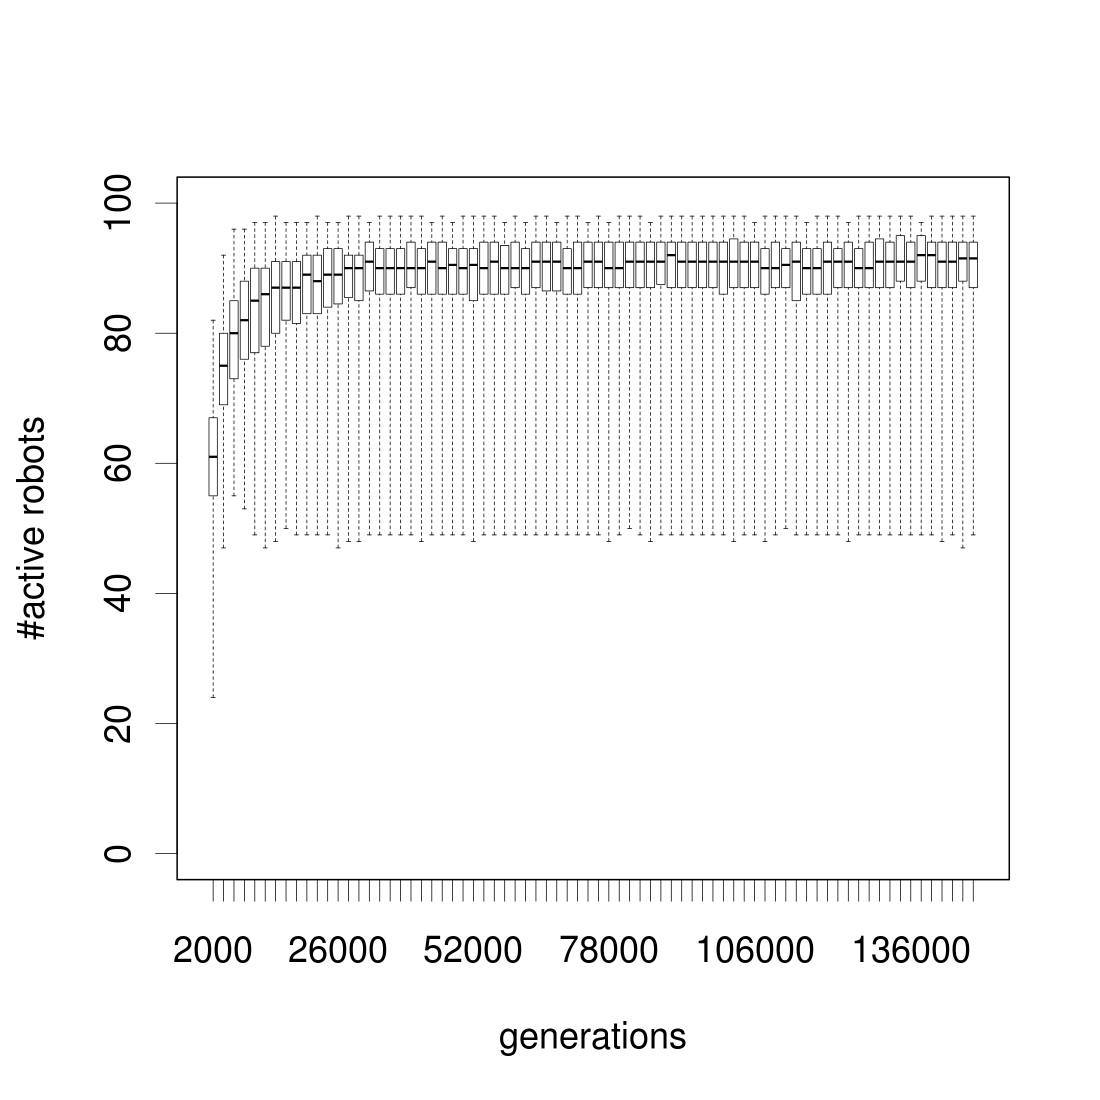
\includegraphics[width=.25\textwidth]{../images/5StaticEnv/alive_staticEnv1}
\end{figure}


\item \begin{lstlisting}[language=R]
plotGandReward(data[data$Sim == 10,],data_active[data_active$Sim == 10,],lwd=1,col=F)
	#lwd=1 : la largeur des points
	#col=F pas de couleur associe a la position des points
\end{lstlisting}
Qui affiche l'évolution de $g_{skill}$ en fonction du temps.
Data doit contenir \verb?read.csv("logs_genometracking.csv")? et \verb?data_active?\verb?read.csv("logs_actives.csv")?.
Exemple du resultat :
\begin{figure}[H]
\center
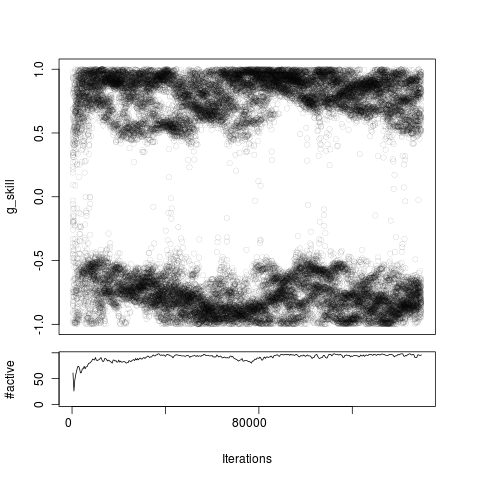
\includegraphics[width=.25\textwidth]{../images/5StaticEnv/Gplot58_staticEnv1}
\end{figure}

Peut être appeler par un fonction de plus haut niveau : \verb?drawAllGraph(data,height,width)? qui permet d'ecrire les graphes de toutes les simulations contenue dans data.


\item \begin{verbatim}
plotGFixed(data[data$Sim == 10,])
\end{verbatim}
Permet d'afficher le $g_{skill}$ de chaque robot pendant toute la simulation 10. Data doit contenir \verb?read.csv("logs_genometracking.csv").? Exemple du resultat : 
\begin{figure}[H]
\center
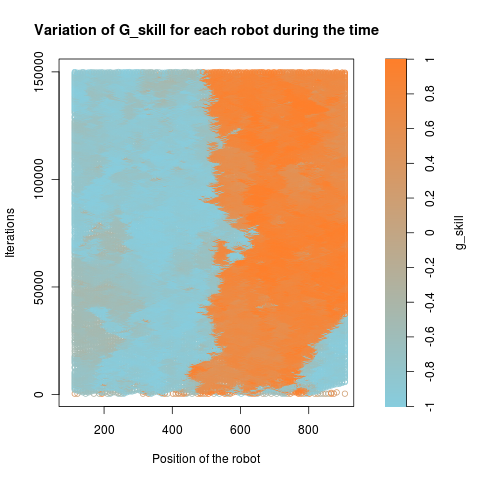
\includegraphics[width=.25\textwidth]{../images/5StaticEnv/Gplot58Static_staticEnv1}
\end{figure}

Peut être appelé par une fonction de plus haut niveau : \verb?drawAllFixed(data,height,width)? qui permet d'ecrire les graphes de toutes les simulations contenue dans data.

\item \verb?reward(g_skill,type,n,b)? qui retourne l'energie recolter par un robots en fonction de son $g_{skill}$, du type de la ressource $\{0,1\}$ est des gProperties $n$ et $b$. Très utile indirectement via les fonctions :

\item \verb?plotReward(n,b,ressourceValue)? qui affiche les deux courbes de recolte pour les deux ressources en fonction de $g_{skill}$, des paramètres $n$ et $b$ (gN et gB) et de la valeur max d'une recolte (ie $gEnergyPointValue$).
\begin{figure}[H]
\center
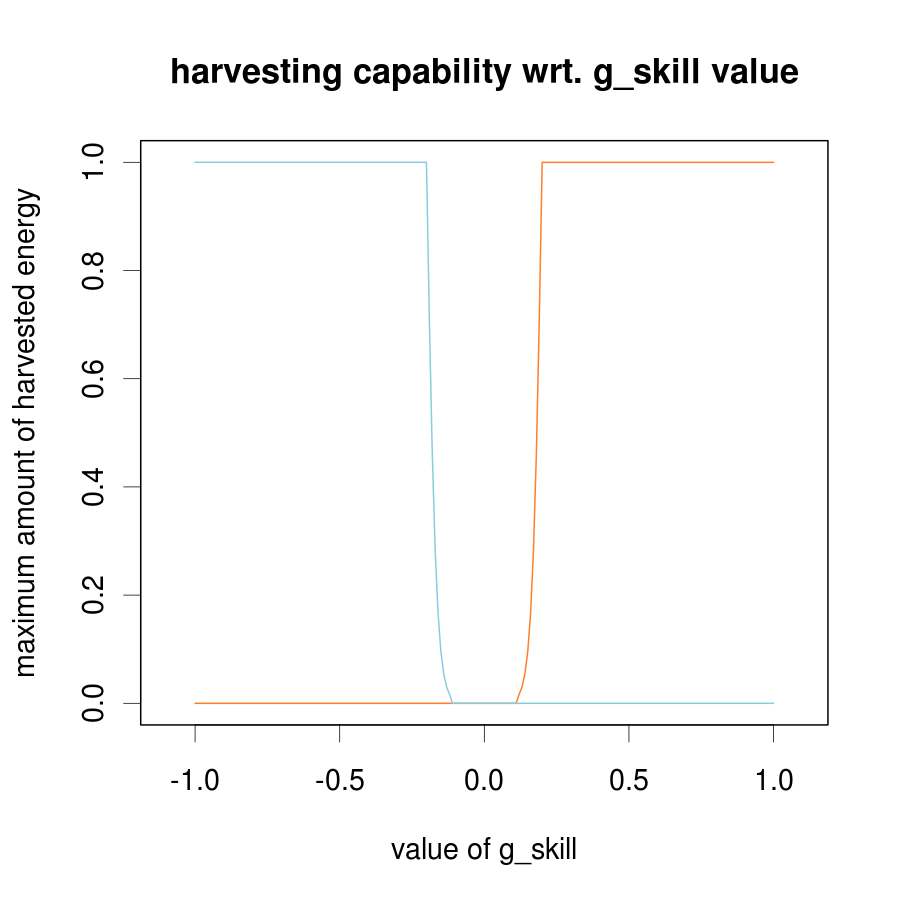
\includegraphics[width=.25\textwidth]{../images/sparsityEffect/f_skill}
\end{figure}


\item \verb?my3dwire(data,ressource,fun,normalized)? : Qui permets de faire un graph en 3dimension avec le nombre de robots actif utilisant une ressource donnée en fonction de la sparsité et de la repartition d'une ressource.
Data doit contenir : \verb? read.csv("logs_actives.csv")?, $ressource \in \{"r0","r1","both","alive"\}$, qui permet de preciser l'affichage du nombre de robots utilisant quelle ressource on veut (alive signife tout les robots peut importe la ressource qu'il utilise). Fun une fonction à appliquer aux donnés (exemple : mean ou median). Si $normalized=TRUE$ le nombre d'actif sur une ressource sera normaliser par le nombre d'actif total (à ne pas faire donc si $ressource="alive"$)

\textcolor{red}{Necessite la librarie : \verb?library(lattice)? de chargée (juste tapper \verb?library(lattice)? pour la charger.  Si elle n'est pas installée : \verb?install.packages("lattice")?


Exemple :
\begin{figure}[H]
\center
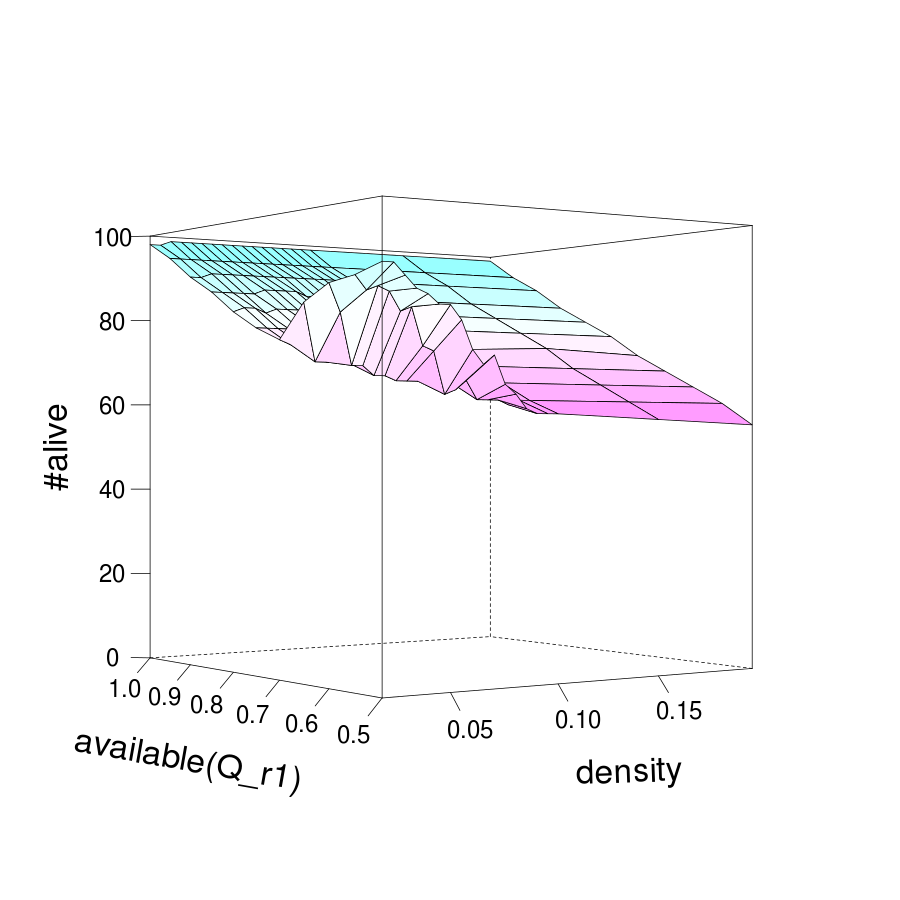
\includegraphics[width=.25\textwidth]{../20110914-Specialisation-FirstNote/images/active_median}
\end{figure}



\end{itemize}




\subsection{Affichage du reseau}
Pour afficher le réseau de communication il est possible d'utiliser les outils de la suite libre GraphViz (sudo apt-get install graphviz). Le script \url{Roborobo/pers/simon/sparsity/drawAllNetworks.sh} permets d'écrire sous forme d'image png l'ensemble des fichiers .dot d'un dossier. ex:
\begin{lstlisting}[language=bash]
./drawAllNetworks ${DIR} ${TOOLS} ${TARGET}
./drawAllNetworks logs neato images
\end{lstlisting}
\begin{itemize}

 \item \$\{DIR\} : un dossier avec des fichier .dot,
 \item \$\{TOOLS\} : un outils de la suite GraphViz \{neato|circo|twop|...\}
 \item \$\{DEST\} : un dossier dans lequel seront stockés les fichiers images png (allGraph si rien)
\end{itemize}





\chapter{Grid 5000}

\section{Avant tout}
\label{sec:gnl}
{
\itshape
\small
---Tout ce qui concerne le fonctionnement general de grid5000 est décrit : \url{http://www.grid5000.fr/mediawiki/index.php/Understanding_Grid5000}, la lecture du très bon readme de JM est aussi conseillée : \url{evorob/Dev/Roborobo/perso/jeanmarc/grid5000/README} ---\\
 
}

Récupérer une image et le .env qui va avec (disponible ici : \url{/users/tao-nosave/jmontani/roboroboImage.tgz} ou encore ici :\url{/users/tao-nosave/carrignon/roboroboImage.tgz}, avec mEDEA-sp à jour pour la seconde image ); et les mettre dans un répertoire dans son espace personnel sur le frontend. Ensuite \emph{!modifier le .env pour que l'adresse de l'image corresponde!}.
Une fois cela fait pour mettre à jours l'image voir la section \ref{sec:maj}.

\section{Accès aux frontend}
\label{sec:frontend}
D'abord se connecter sur l'access d'un site puis à son frontend (depuis lequel il est possible d'avoir accès et de réserver des noeuds)
\begin{lstlisting}[language=bash]
ssh user@access.grenoble.grid5000.fr
ssh frontend
\end{lstlisting}
Le site (ici grenoble par affinité) peut être remplacé par n'importe quel site de grid5000 (orsay,lille,rennes,reims,lyon,...).



\section{Reservation/deploiement (en mode interactif)}
\label{sec:reserv}
Pour reserver \$n noeuds pendant \$h heures :

\begin{lstlisting}[language=bash]
oarsub -I -l nodes=$n,walltime=$h -t deploy
\end{lstlisting}


Suite à quoi l'utilisateur est directement connecté sur son job et peut acceder entres autres, aux variables :

\begin{lstlisting}[language=bash]
$OAR_JOBID #l'id du job
$OAR_FILE_NODES #le nom de tous les noeuds disponibles pour ce job
\end{lstlisting}
Le deploiement de l'environnement se fait ensuite simplement en utilisant la commande :
\begin{lstlisting}[language=bash]
kadeploy3 -f $OAR_FILE_NODES -a roborobo.env

\end{lstlisting}

\section{Lancement des expériences / récupération des données}
\label{sec:run}
Un très bon outils développé par jm.montanier est disponible (cf : \url{evorob/Dev/Roborobo/perso/jeanmarc/grid5000/README} ; qui permet de lancer et de rappatrier les expériences d'une traite en s'appuyant sur des tunnels ssh en ne passant pas par le mode interactif (ce qui permet d'éviter d'avoir à être présent pour le déployement)

Sinon il faut :
\begin{enumerate}
 \item Reserver et déployer le nombre de noeuds voulus (cf section \ref{sec:reserv}),
 \item Lancer chaque expérience sur chaque noeud depuis le frontend,
 \item récupérer les logs sur le frontend une fois les expériences finies,
 \item envoyer les logs depuis access sur une machine "hors grille" (ie pl-ssh.lri.fr par exemple)
\end{enumerate}

\subsection{Les scripts}
Les scripts testDifferencesRessourceCap.sh et bringBackAllLogs.sh, disponibles dans \url{evorob/Dev/Roborobo/perso/simon/grid5000/} permettent d'automatiser les points 2 et 3 mais de fa\c con assez spécifique à l'étude de la sparsitée. Le premier permet de lancer depuis le frontend sur chaque noeud une série d'expériences pour un ensemble de valeur de $gNbAllowedRobotBySun$. Le second permet de ramener tout les logs générés par le premier sur le frontend. 

De fa\c con plus détaillée :
\begin{lstlisting}[language=bash]
 ./testDifferencesRessourceRepartition.sh START END STEP
\end{lstlisting}
\begin{itemize}
 \item START : the first repartition
 \item END : the last reparition 
 \item STEP : LE pas entre chaque repartition testée
\end{itemize}
Envoie sur les chaque noeud reservé un script (actuellement le script ./testAllSparsity cf. section \ref{sec:scriptextract}) avec différentes répartition des ressources.
Attention : il faut qu'il y ai suffisament de noeuds reservés pour pouvoir tester toutes les répartitions entre start et end avec le pas step! (ie $length(seq(start,end,step)))<=Nb_{Noeuds}$)

Pour chaque noeud un fichier de log avec le nom du noeud est écrit dans lequel est redirigée la sortie standard du noeud (c'est a dire l'output de ./testAllSparsity). 

Ensuite les dossiers de logs sont compressés à l'aide de la commande bunzip.
Les paramètres données à ./testAllSparsity son codés en dur dans le script


Exemple :
\begin{lstlisting}[language=bash]
./testDifferencesRessourceRepartition.sh 1 95 5 
\end{lstlisting}
va executer sur 20 noeuds le script ./testAllSparsity avec les répartations 1/99, 6/94, 11/89 ..., 91/9 . 


Une fois terminée et que toutes les commandes ont été exécutées, on peut lancer ./bringBackAllLogs, sans arguments, qui recupère tout les zips des logs et les rappatrie dans le home du frontend.\\


\textbf{Pour résumer :}

\begin{lstlisting}[language=bash]
oarsub -I -l nodes=$n,walltime=$h -t deploy
kadeploy3 -f $OAR_FILE_NODES -a roborobo.env
./testDifferencesRessourceRepartition.sh 1 95 5 
#attendre de voir sur tout les fichiers de logs "jobdone."
./bringBackAllLogs
\end{lstlisting}
une bonne sécurité est d'effectuer l'ensemble de ces manips depuis un screen (screen -S allExp) que l'on peut acceder depuis d'autres endroits sans clore le jobs.\\

Ensuite les données peuvent-être rappatriées à la maison pour être analysées (cf. chapitre \ref{ch:script}) :
\begin{lstlisting}[language=bash]
** Sur grid5000
scp *.tbz user@pl-ssh.lri.fr:~
** sur pl-ssh:~
tar xjvf *.tbz
for i in * ; do
	./followaGene.sh 1 1500 $i/logs $i
done

\end{lstlisting}

\textbf{il manque un script pour concatener toutes les experiences, en cours de réalisation et d'utilisation}

\section{Modification MAJ de l'image}
\label{sec:maj}

Pour modifier l'image / mettre à jour Roborobo il faut :
\begin{enumerate}
 \item Copier le dossier Roborobo (vidé de tout élément inutile, make clean, etc... c'est le dossier qui sera ensuite redéployé à chaque fois pour chaque expérience) sur access  
\begin{lstlisting}[language=bash]
scp -r Roborobo username@access.grenoble.grid5000.fr
\end{lstlisting}
\item reserver un noeud en mode interactif et déployer l'image non encore à jour dessus:
\begin{lstlisting}[language=bash]
oarsub -I -l nodes=n,walltime=h -t deploy #reservation
kadeploy3 -f $OAR_FILE_NODES -a roborobo.env #deployement
\end{lstlisting}
\item Mettre à jour le dossier sur le noeud
\begin{lstlisting}[language=bash]
ssh root@`cat $OAR_FILE_NODES | uniq` #ou ssh root@nomdunoeud
\end{lstlisting}
créer un dossier ou supprimer le dossier qui va être mis à jour puis se déconnecter. Ensuite, copier le dossier Roborobo du frontend sur le noeud déployé:
\begin{lstlisting}[language=bash]
scp -r Roborobo root@`cat $OAR_FILE_NODES | uniq`:~/dest
#ou scp ... root@nomdunoeud
\end{lstlisting}
puis se reconnecter au noeuds et recompiler roborobo :
\begin{lstlisting}[language=bash]
ssh root@`cat $OAR_FILE_NODES | uniq` #ou ssh root@nomdunoeud
cd folderfith/Roborobo
make #make clean si pas 
     #fait avant l'envoie depuis la machine perso
\end{lstlisting}

\item et générer une image grâce à la commande :

\begin{lstlisting}[language=bash]
ssh root@genepi-8 tgz-g5k > roboroboImage.tgz
\end{lstlisting}
Commande qui n'output rien si ce n'est quelques warnings ; c'est normal.



\end{enumerate}





\end{document}

